\section{Introductie}


\subsection{Aanleiding en Context}

Voortman Machinery, gevestigd in Rijssen is producent van geavanceerde metaalbewerkingsmachines. In het begin richtte Voortman zich vooral op de productie van staalconstructies. In 1995 begon Voortman ook staalbewerkingsmachines te ontwikkelen en te produceren waaruit de naam Voortman Steel Machinery is ontstaan. In de loop der jaren is het bedrijf uitgegroeid tot een wereldwijde fabrikant van \gls{cnc}-staalbewerkingsmachines met hierbij ook de bijpassende softwareoplossingen \cite{web:VoortmanGeschiedenis}. In veel machines van Voortman zitten spindels, deze spindels worden gebruikt in de machines om bijvoorbeeld te vrezen, tapen of boren. Na een bepaalde tijd kunnen deze spindels door slijtage of schade niet meer correct functioneren. Ze kunnen dan in veel gevallen nog gereviseerd worden door de fabrikant, dit kan echter veel geld kosten.
 
\vspace{0.5cm}
 
  Voortman wil daarom de spindels zelf kunnen reviseren en hebben hiervoor een testkast ontwikkeld om de spindels die zij gebruiken te testen. Echter ondersteunt deze kast (figuur \ref{fig:TestKastFoto}) bij Voortman slechts één soort spindel terwijl er wel veel verschillende soorten spindels gebruikt worden in het machine portfolio van Voortman. Hieruit kwam de opdracht om de testkast aan te passen zodat zo veel mogelijk soorten spindels kunnen worden getest op de testkast van Voortman zelf.
  
\vspace{0.5cm}

Om dit probleem op te lossen, wordt in dit verslag onderzocht hoe de testkast kan worden aangepast. Hoofdstuk \ref{sec:ProbleemAnalyseEnEisen} in dit verslag gaat in op de huidige situatie, de problemen en de eisen van de testkast. Hoofdstuk \ref{sec:TheoretischKader} gaat verder in op de eisen en de ontwerpmogelijkheden. Waar hoofdstuk \ref{sec:Implementatie} en \ref{sec:Uitbreidingen} over de implementatie van het ontwerp gaan. Tot slot beschrijft hoofdstuk \ref{sec:Testen} de testen en de resultaten van de testkast na de verbeteringen.

\begin{figure}[h]
	\centering
	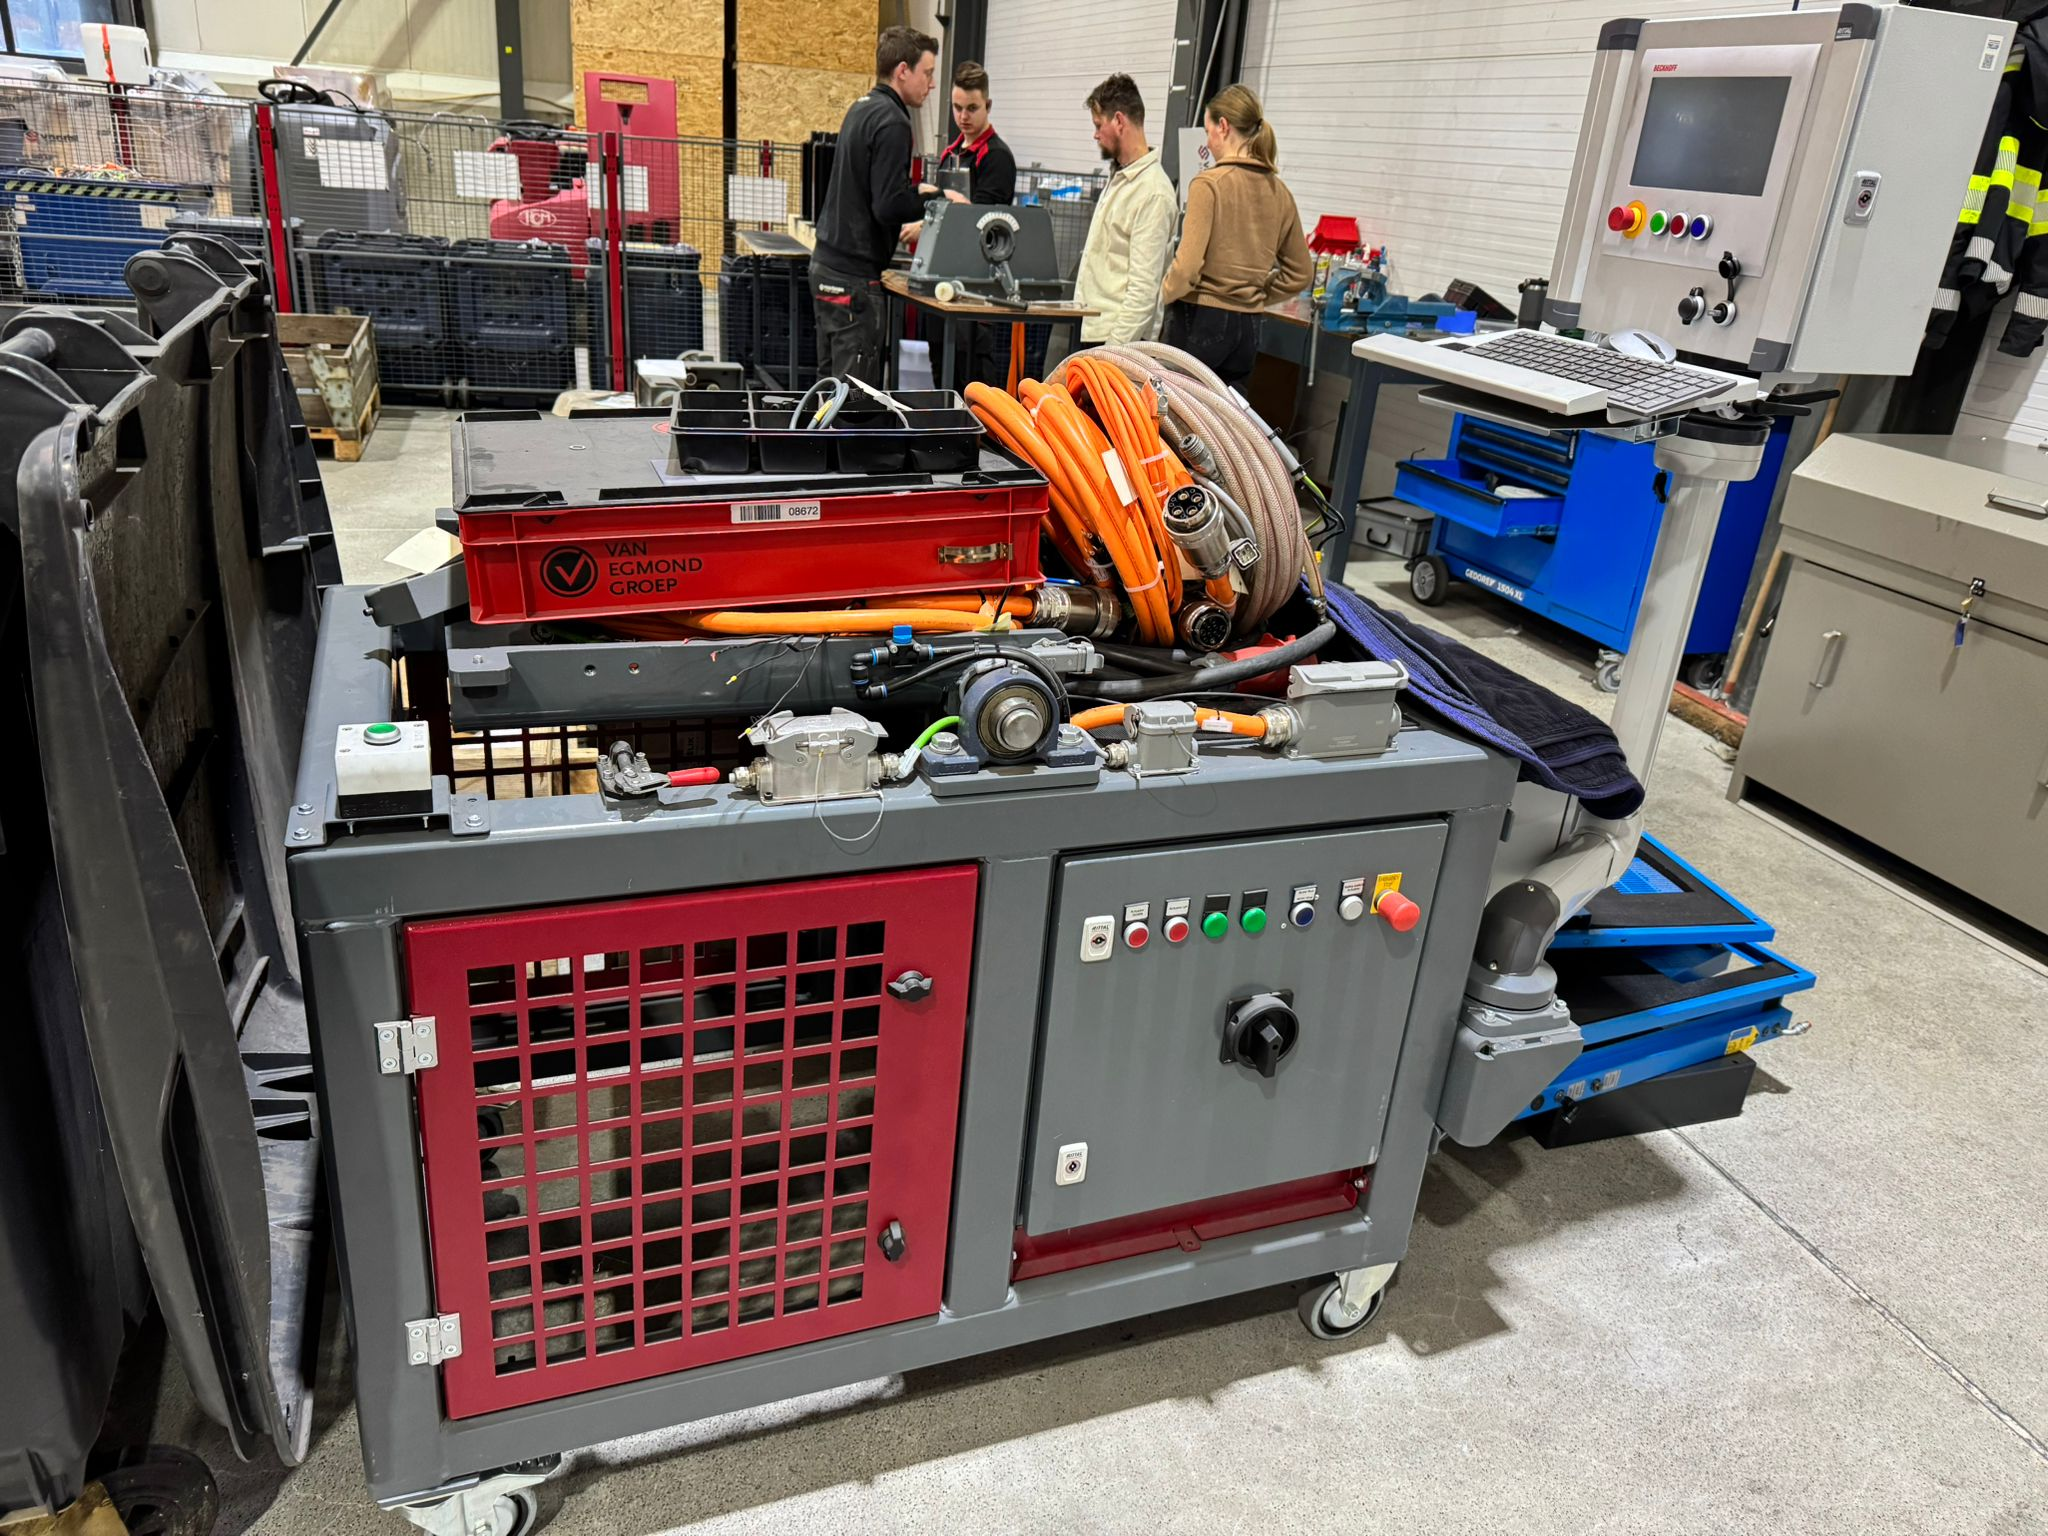
\includegraphics[width=250pt]{TestKast}
	\label{fig:TestKastFoto}
	\caption{Foto van de bestaande testkast}
\end{figure}

\newpage

\subsection{Doelstelling}

Op het moment zit er een Beckhoff \gls{AX5140} servo drive in de testkast gebouwd voor het aansturen van de motoren. De parameters die in deze drive zitten kunnen momenteel alleen de servomotor HQL100X aansturen. Andere motoren kunnen niet worden aangestuurd met deze parameters omdat deze motoren bijvoorbeeld een andere encoder hebben, andere \gls{pid}-instellingen of de motor werkt simpelweg volgens een ander principe (asynchrone of synchrone servo). De \gls{AX5140} heeft meer dan 400 parameters de meeste hiervan kunnen worden aangepast.

\vspace{0.5cm}

Ook is het testprotocol van Voortman op de spindels niet erg geavanceerd zo worden motoren alleen aangestuurd naar een bepaald tourental voor een bepaald aantal seconden waarbij er gelet wordt of de motor niet te veel trilt en of deze niet te warm wordt. Zij kwantificeren deze waardes niet het is daarom erg lastig om aantoonbaar de motor te beoordelen op zijn prestaties.

\vspace{0.5cm}

De wens is daarom vanuit Voortman om uit te zoeken welke parameters relevant zijn voor wanneer er een motor gewisseld wordt en welke waardes dit moeten zijn voor de motoren die zij willen gaan testen. Met daarbij een programma die ervoor kan zorgen dat deze parameters eenvoudig naar de drive kunnen worden geschreven. Daarnaast moet er uitgezocht worden wat Voortman wil gaan testen aan de motoren en wat hiervoor eventueel voor nodig is zoals een trilling sensor die de trillingen van de spindel kan meten.

\newpage

\subsection{Onderzoeksvragen}

Tijdens de afstudeerperiode zullen de volgende onderzoeksvragen beantwoord worden:

\begin{enumerate}
	\item Welke specifieke motorparameters zijn noodzakelijk om minimaal 90\% van de door Voortman gebruikte motortypes aan te sturen en hoe kunnen deze parameters binnen zes weken worden geïdentificeerd?
	
	\item Hoe kunnen motorparameters automatisch geschreven worden naar de drive, en hoe kan dit binnen zes weken worden geïmplementeerd en getest voor tenminste drie motortypes?
	
	\item Welke encoderinterfaces (e.g. \gls{SSI} of EnDat) zijn noodzakelijk om 90\% van de door Voortman gebruikte motoren te ondersteunen op de testkast, en hoe kunnen deze interfaces binnen zes weken worden getest op te testkast.
	
	\item Welke meetmethodes en testcriteria (e.g. temperatuur, stroomverbruik toerental en trillingen) kunnen worden gebruikt om minimaal 90\% van de potentiële defecten in gereviseerde motoren te detecteren, en hoe kan een testprotocol binnen acht weken worden opgesteld en gevalideerd?
	
	\item Hoe kan de software op de testkast binnen acht weken worden geprogrammeerd om automatisch testresultaten te loggen, waarbij afwijkingen in bijvoorbeeld trillingen of overbelasting kunnen worden gedetecteerd en gerapporteerd in een gestructureerd \gls{PDF}-rapport.
	
	\item Welke software of hardware aanpassingen zijn er nodig om binnen drie maanden een modulaire testomgeving te onwikkelen, waarbij nieuwe motortypes zonder codewijzigingen en een maximale configuratie tijd van maximaal één uur kunnen worden toegevoegd?
\end{enumerate}

\newpage

\subsection{Afbakening}

\subsubsection{Belangrijkste doelstelling}

Voortman heeft er in eerste instantie het meeste belang bij dat er meer spindels op de testkast kunnen worden getest daarom zal de prioriteit van dit onderzoek liggen bij het uitbreiden van de testmogelijkheden van de testkast voor verschillende spindels (Onderzoeksvraag 1 en 2).

\subsubsection{Aannames en Uitgangspunten}

Voor dit onderzoek wordt aangenomen dat de huidige motordrive op de testkast geschikt is voor de motoren die Voortman wil gaan testen op de testkast. Dit houdt in dat de drive alle benodigde encoderinterfaces ondersteunt (of met encoder option card) en dat alle motoren fysiek aangesloten kunnen worden met bestaande bekabeling en aansluitingen.

\vspace{0.5cm}

Deze aannames zijn gebaseerd op informatie van eerdere onderzoeken en interne specialisten binnen Voortman. Indien tijdens de implementatie toch blijkt dat bepaalde motoren niet aangesloten kunnen worden op de testkast, zal er onderzocht worden welke aanpassingen nodig zijn om dit alsnog mogelijk te maken en dit zal dan als dit mogelijk is ook worden gerealiseerd. Deze aanpassingen vallen echter buiten de oorspronkelijke scope van dit onderzoek, maar kunnen indien nodig in de aanbevelingen worden opgenomen.

